\documentclass[aspectratio=169,fleqn]{beamer}
\PassOptionsToPackage{english}{babel}
\usepackage{standardslides}


\setbeamertemplate{footline}[frame number]
\setbeamertemplate{navigation symbols}{}
\setbeamertemplate{background}{
  
\includegraphics[width=\paperwidth,height=\paperheight]{images/background-tessellation.png}
}

\title{Curve Smoothing on Surface Meshes}
\author{Markus Pawellek}

\bibliography{references}

\begin{document}

\selectlanguage{english}

\frame[plain]{\titlepage}
% \begin{frame}[plain]{Outline}
%   \footnotesize
%   \hfill\parbox[t][7cm][l]{0.9\textwidth}{\tableofcontents}
% \end{frame}

\setcounter{framenumber}{0}

\section{Introduction and Background}

  \begin{frame}{Introduction and Background: Reference}
    \centering
    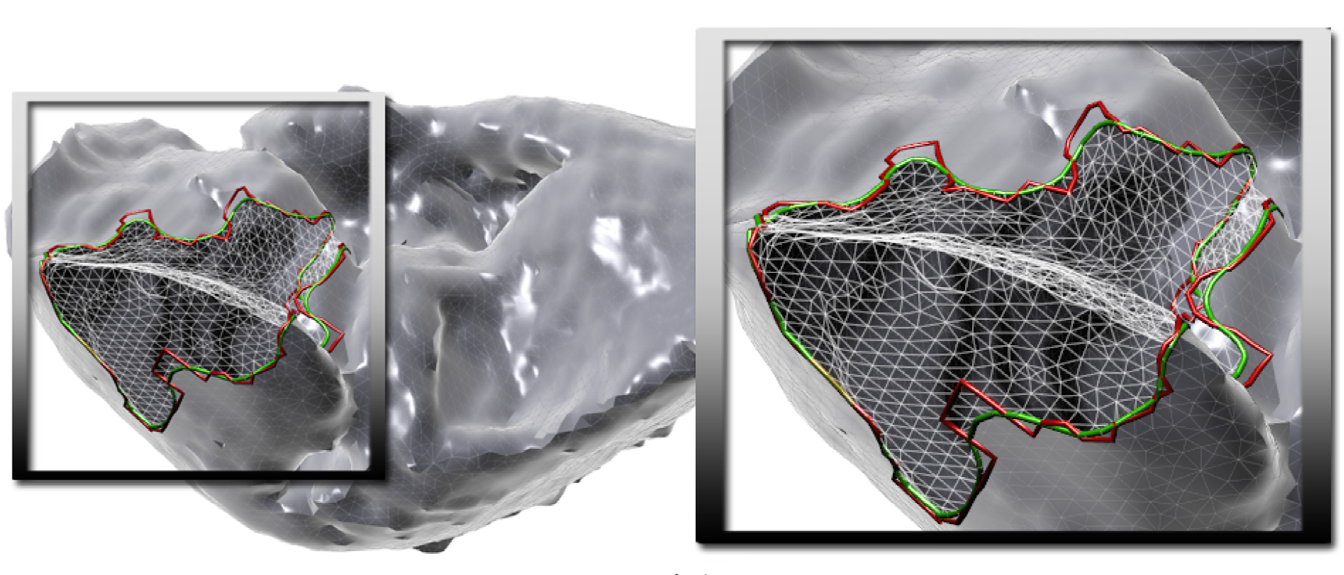
\includegraphics[width=0.66\linewidth]{images/lawonn2014-2.png}
    \hfill
    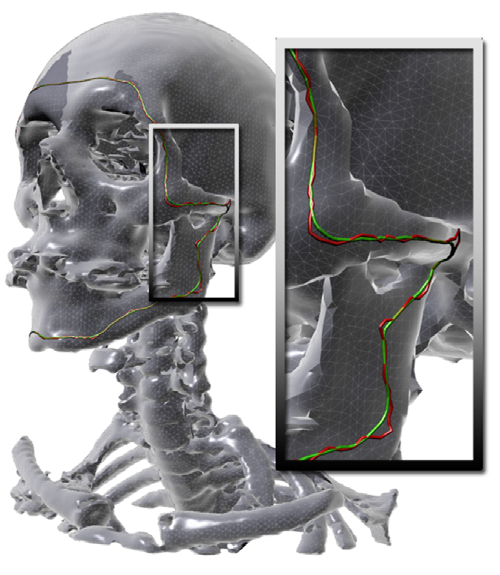
\includegraphics[width=0.24\linewidth]{images/lawonn2014-1.png}

    \bigskip
    \fullcite{lawonn2014}
  \end{frame}

  \begin{frame}{Introduction and Background: Goals}
    \begin{minipage}[c]{0.45\linewidth}
      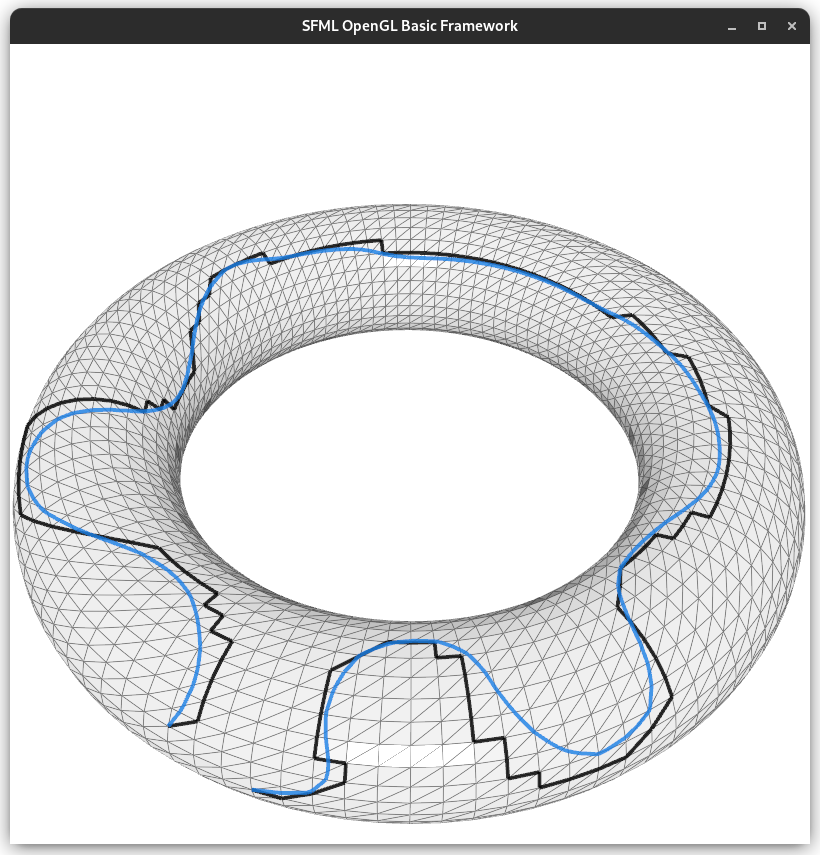
\includegraphics[width=\linewidth,trim={15px 20 15 50},clip]{images/torus-smooth-0.95.png}
    \end{minipage}
    \hfill
    \begin{minipage}[c]{0.45\linewidth}
      \pause
      \begin{itemize}
        \item<+-> Closeness to Initial Curve
        \item<+-> Balancing Closeness and Smoothness by Parameter
        \item<+-> Proof of Convergence and Smoothness
        \item<+-> Robust toward Geometric and Parametric Noise
      \end{itemize}
    \end{minipage}
  \end{frame}

  \begin{frame}{Introduction and Background: Implementation}
    \begin{minipage}[c]{0.45\linewidth}
      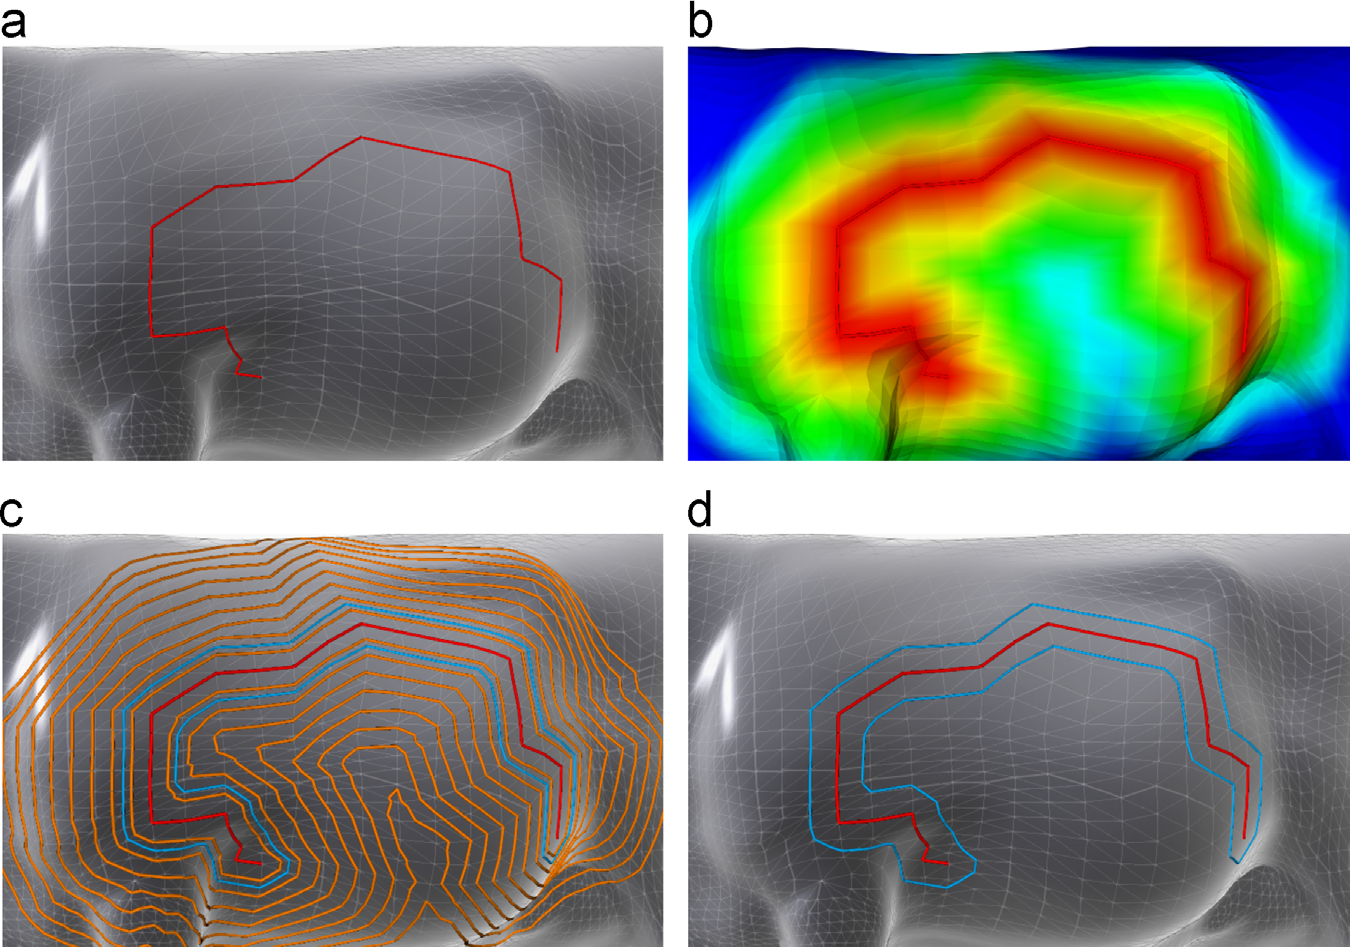
\includegraphics[width=\linewidth]{images/lawonn2014-3.png}
    \end{minipage}
    \hfill
    \begin{minipage}[c]{0.45\linewidth}
      \pause
      \begin{itemize}
        \item<+-> Distance Envelope
        \item<+-> Weighted Relaxation of Geodesic Curvature to Desired Geodesic Curvature
        \item<+-> Convergence based on Length Reduction
      \end{itemize}
    \end{minipage}
  \end{frame}

\section{The Idea}
  \begin{frame}{The Idea: Surfaces in 2D}
    \begin{minipage}[c]{0.45\linewidth}
      \only<1-2>{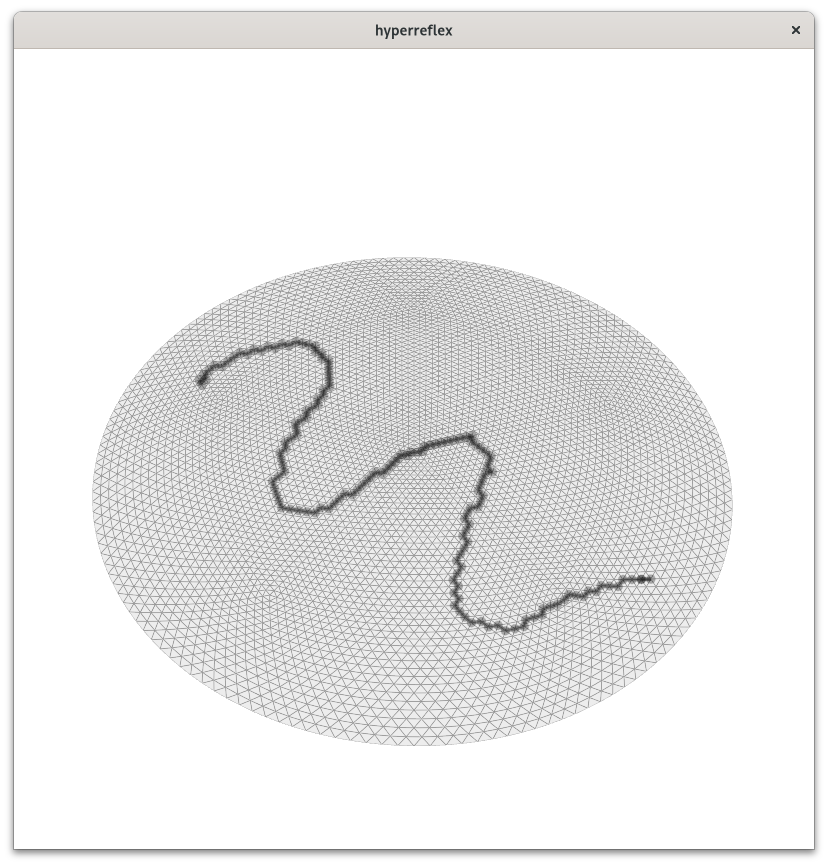
\includegraphics[width=\linewidth,trim={20px 20 20 50},clip]{images/circle-01.png}}%
      \only<3>{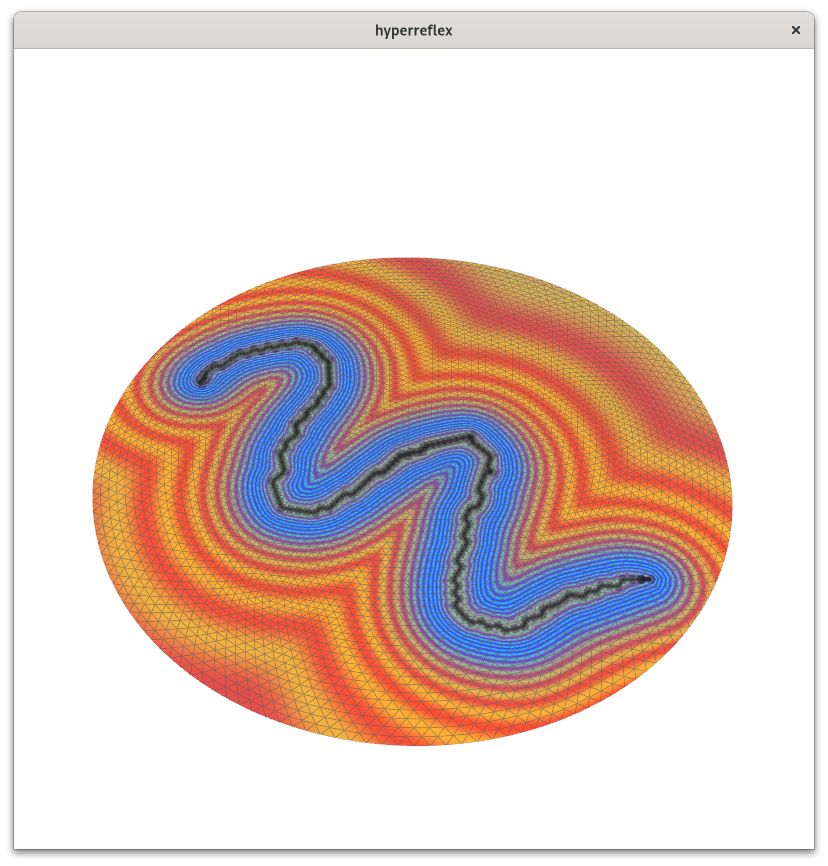
\includegraphics[width=\linewidth,trim={20px 20 20 50},clip]{images/circle-02.png}}%
      \only<4>{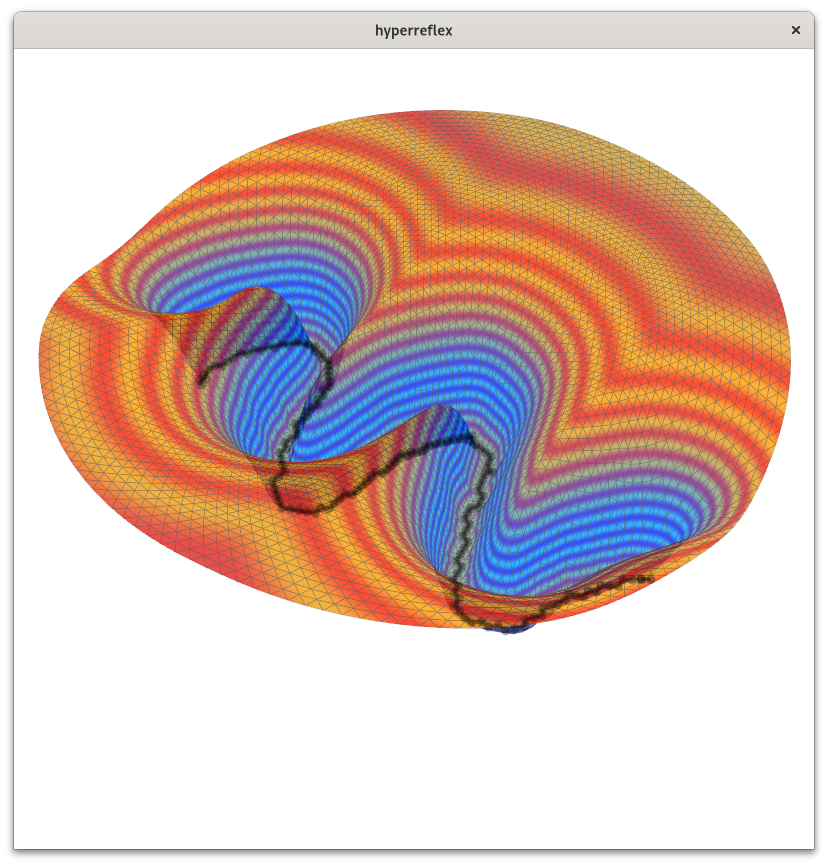
\includegraphics[width=\linewidth,trim={20px 20 20 50},clip]{images/circle-03.png}}%
      \only<5>{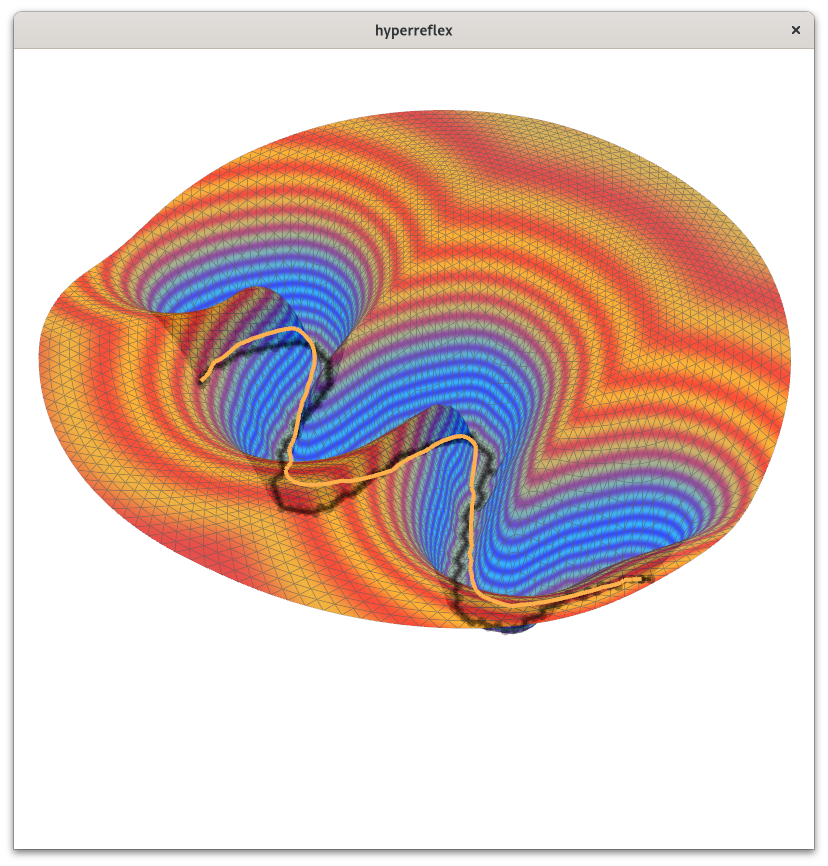
\includegraphics[width=\linewidth,trim={20px 20 20 50},clip]{images/circle-04.png}}%
      \only<6>{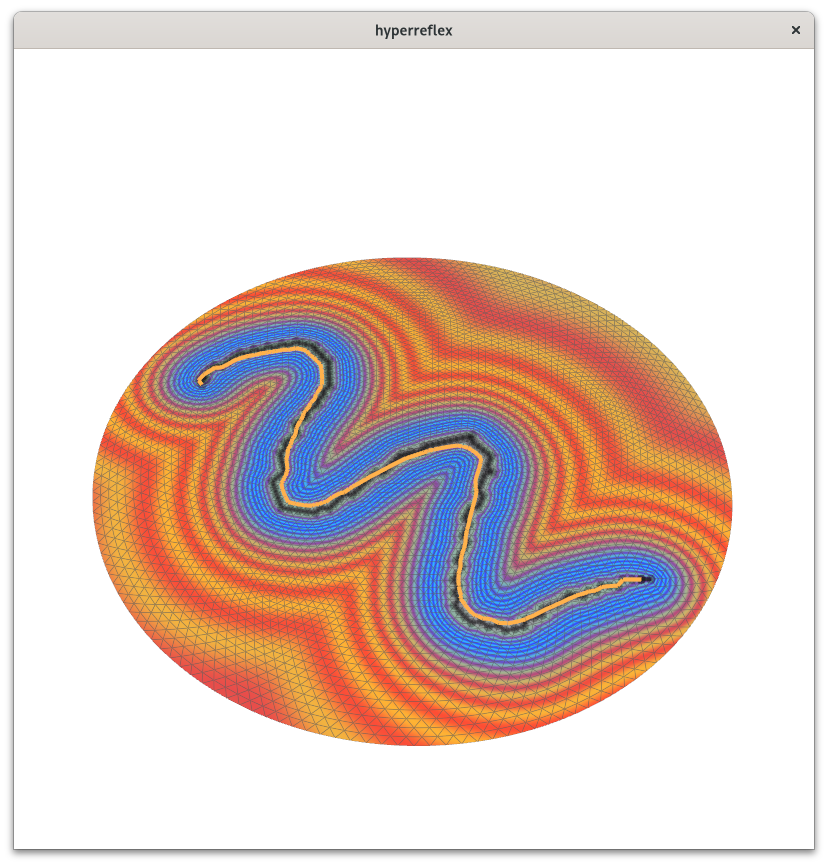
\includegraphics[width=\linewidth,trim={20px 20 20 50},clip]{images/circle-05.png}}%
      \only<7>{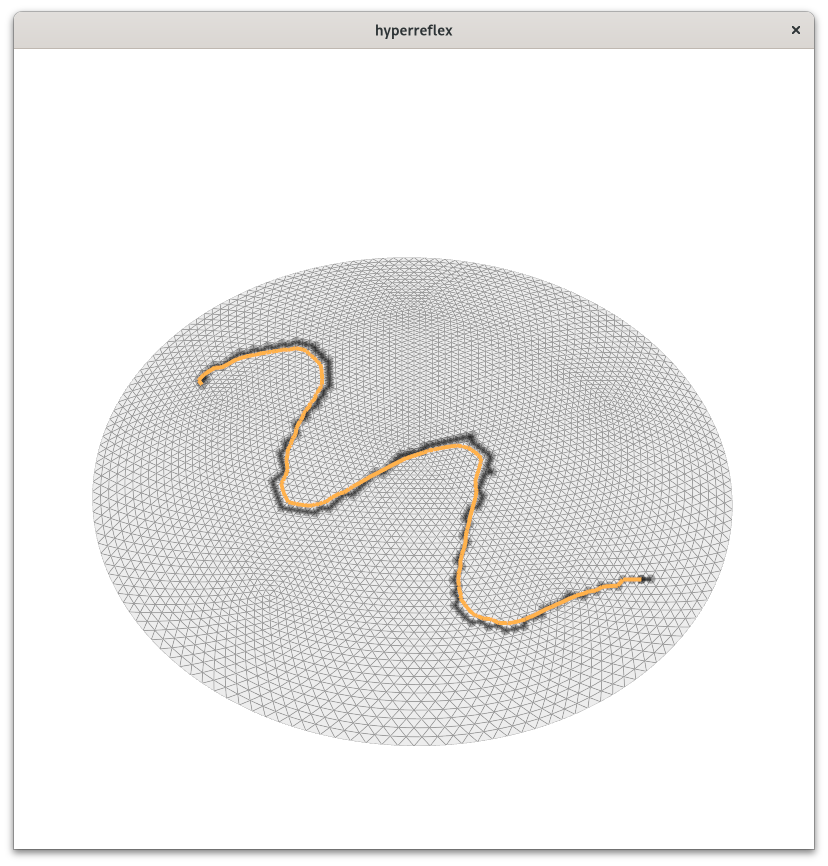
\includegraphics[width=\linewidth,trim={20px 20 20 50},clip]{images/circle-06.png}}%
    \end{minipage}
    \hfill
    \begin{minipage}[c]{0.45\linewidth}
      \pause
      \begin{enumerate}
        \item<+-> Start with initial curve
        \item<+-> Generate distance field \\ and penalty potential
        \item<+-> Lift surface to 3D by adding potential to coordinates
        \item<+-> Generate geodesic \\ for lifted surface
        \item<+-> Project geodesic back \\ to original surface
      \end{enumerate}
    \end{minipage}
  \end{frame}

  \begin{frame}{The Idea: Surfaces in 3D}
    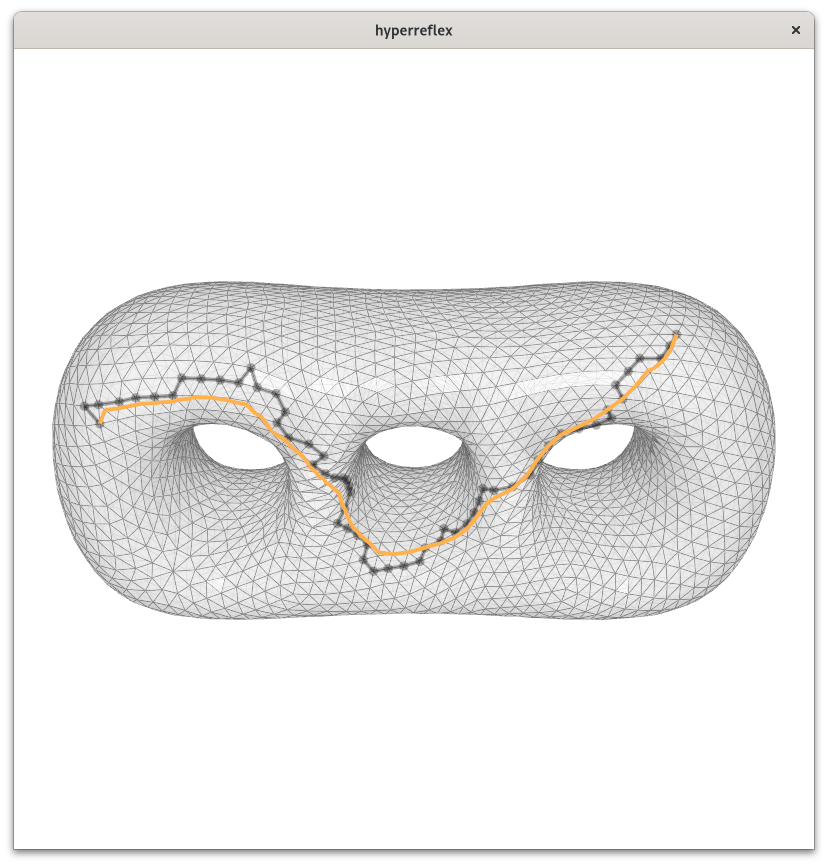
\includegraphics[width=0.45\linewidth,trim={20px 200 20 200},clip]{images/holes-light.png}
    \hfill
    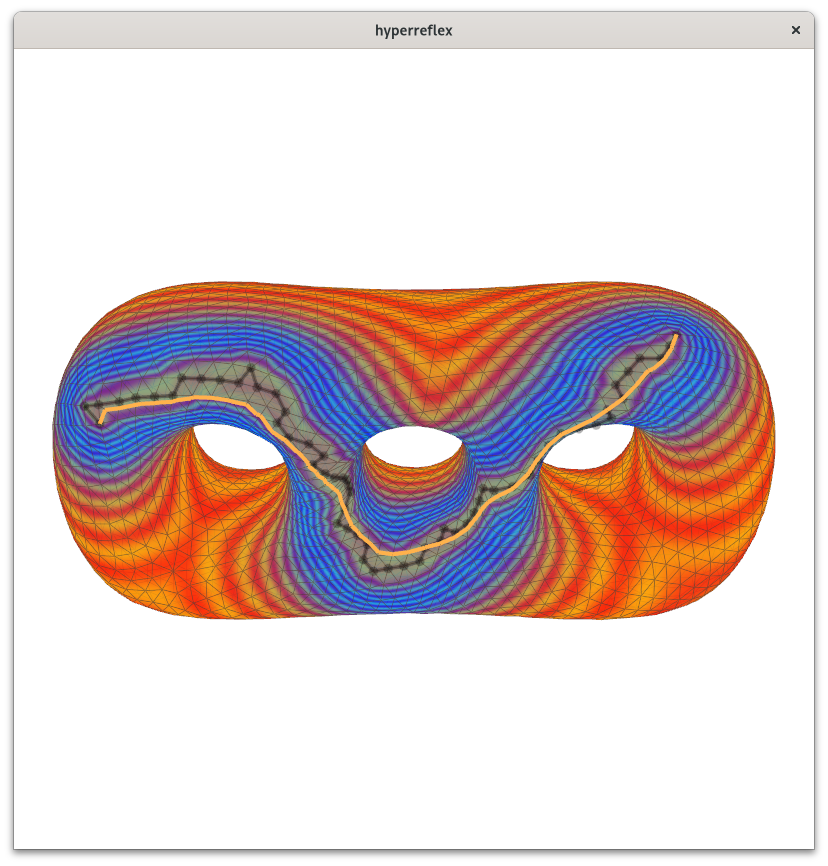
\includegraphics[width=0.45\linewidth,trim={20px 200 20 200},clip]{images/holes-heat.png}

    \bigskip
    \pause
    \begin{itemize}
      \item Surfaces embedded in 3D are lifted into 4D \\ by appending potential to fourth coordinate of vertex positions
    \end{itemize}
  \end{frame}

  \begin{frame}{The Idea: Balancing Closeness and Smoothness}
    \begin{minipage}[c]{0.45\linewidth}
      \only<1-6>{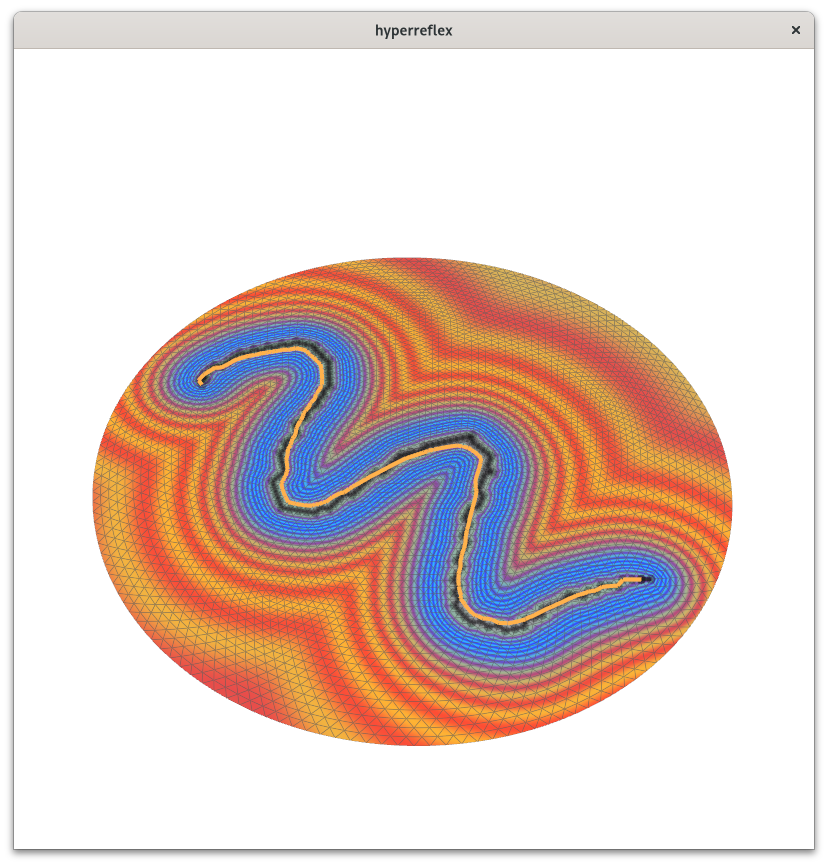
\includegraphics[width=\linewidth,trim={20px 20 20 50},clip]{images/circle-05.png}}%
      \only<7>{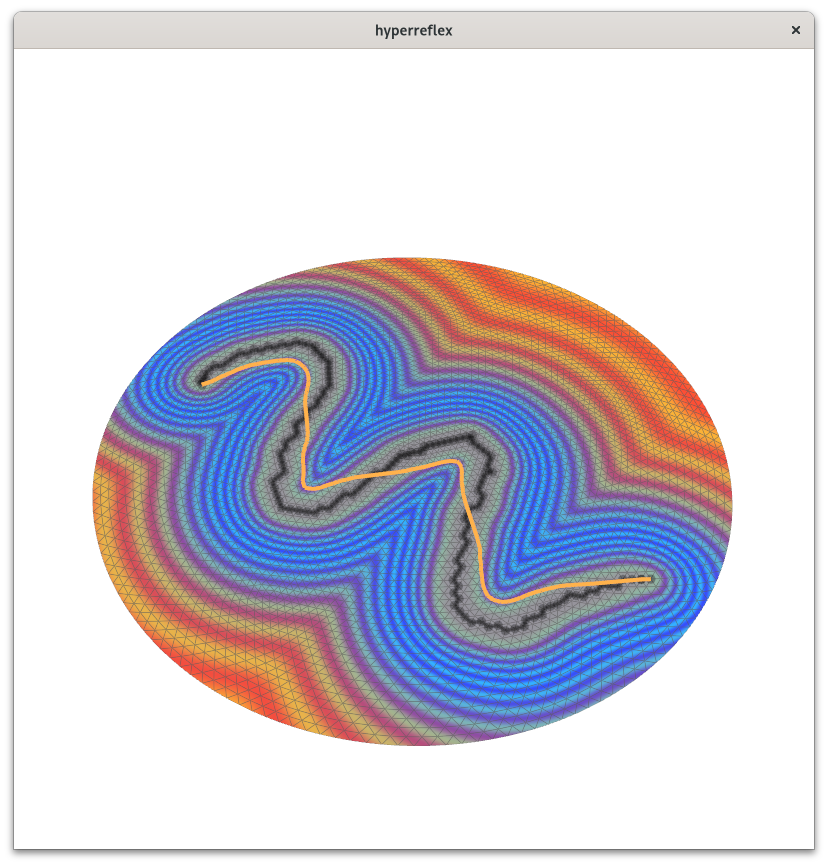
\includegraphics[width=\linewidth,trim={20px 20 20 50},clip]{images/circle-07.png}}%
      \only<8>{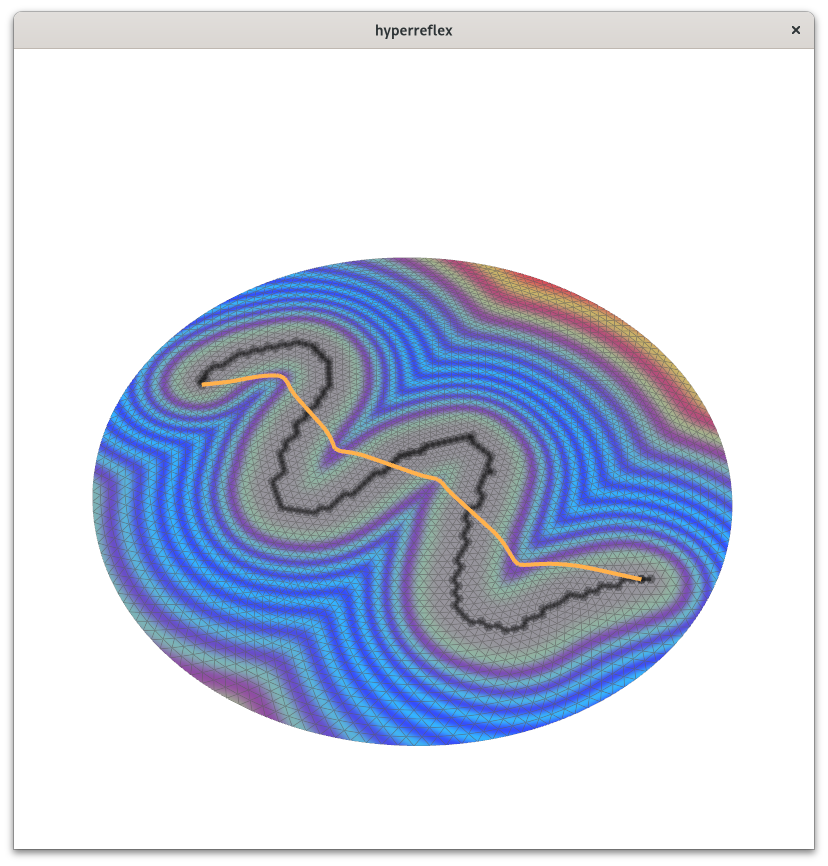
\includegraphics[width=\linewidth,trim={20px 20 20 50},clip]{images/circle-08.png}}%
      \only<9>{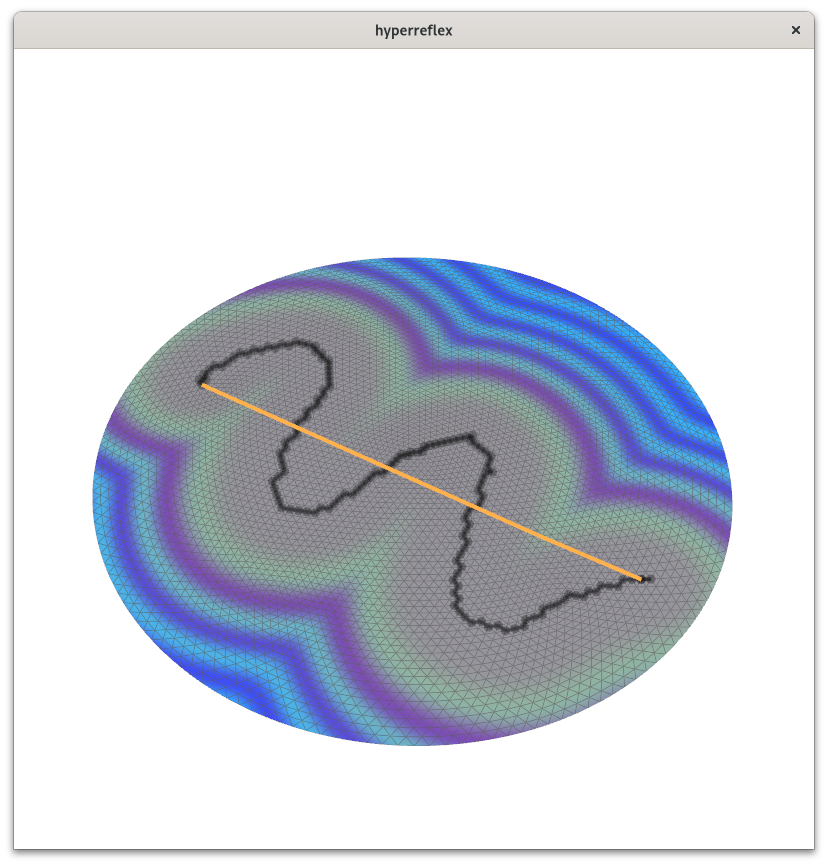
\includegraphics[width=\linewidth,trim={20px 20 20 50},clip]{images/circle-09.png}}%
    \end{minipage}
    \hfill
    \begin{minipage}[c]{0.45\linewidth}
      \pause
      \begin{itemize}
        \item<+-> No restrictions when choosing penalty potentials
        \item<+-> Here, potentials depend on distance $d$ to initial curve
        \item<+-> Using parameterized family of functions allows for balancing
      \end{itemize}

      \pause
      \[
        \function{\varphi_{\alpha,\tau}}{[0,\infty)}{\setReal},\quad \alpha,\tau\in(0,\infty)
      \]
      \[
        \varphi_{\alpha,\tau}(d) \define \alpha\exp\roundBrackets{-\frac{1}{\tau d}}
      \]
    \end{minipage}
  \end{frame}

\section{Properties, Limitations, and Future Work}
  \begin{frame}{Properties}
    \pause
    \begin{itemize}
      \item<+-> Easy implementation
      \item<+-> (Almost) any geodesics algorithm can be used
      \item<+-> Inherits properties from geodesics algorithm (robustness, convergence)
      \item<+-> Preserves closeness by definition
      \item<+-> Other potentials allow for more general movement
      \item<+-> Arbitrarily many parameters
      \item<+-> Potentials may also depend on other surface characteristics, \\ such as mean curvature
    \end{itemize}
  \end{frame}

  \begin{frame}{Limitations and Future Work}
    \pause
    \begin{itemize}
      \item<+-> Scaling of potential
      \item<+-> Good family of penalty potentials
      \item<+-> Enlarging curves
      \item<+-> Measuring smoothness
      % \item<+-> Initial curves with edge vertices
      \item<+-> Further mathematical properties
      % \item<+-> Surface Boundaries
      \item<+-> Applications
      \item<+-> Other References: To best of my knowledge, it has not been done.
      % \item<+-> Performance Improvement: Dynamic Evaluation of Distances
      % \item<+-> Closed Curves
    \end{itemize}
  \end{frame}

\setcounter{backupcounter}{\value{framenumber}}

\setcounter{framenumber}{\value{backupcounter}}

\end{document}
